\section{Geometría Composicional (CoDa) y Tipología Productiva}

% ================================================================
\begin{frame}{Geometría del Simplex: Transformación CLR y PCA}
\vspace{-0.18cm}
\begin{columns}[T,onlytextwidth]
\begin{column}{0.48\textwidth}
\begin{ccdebox}[left=2mm,right=2mm,top=1mm,bottom=1mm]
\scriptsize\RaggedRight
\textbf{1. Cierre Composicional ($\mathcal{S}^D$)}: Las participaciones sectoriales suman $100\%$, induciendo correlaciones negativas espurias en el espacio crudo.\\[0.06cm]
\textbf{2. Reemplazo Multiplicativo}: Lambayeque y San Martín registran $0\%$ en minería (2015--19). Se imputa $\delta = 0.05\%$ reescalando los sectores positivos:
\[
x_{ij}^* = \delta \;\text{(si } x_{ij}=0\text{)}; \quad x_{ij}\!\left(1 - \tfrac{z_i \delta}{100}\right)
\]
\textbf{3. Coordenadas Log-Ratio Centradas (CLR)} con media geométrica $g_i = \big(\prod_{j=1}^D x_{ij}^*\big)^{1/D}$:
\[
\mathrm{clr}(x_i^*) = \left[ \ln\tfrac{x_{i1}^*}{g_i},\, \dots,\, \ln\tfrac{x_{iD}^*}{g_i} \right]
\]
\end{ccdebox}
\end{column}

\begin{column}{0.49\textwidth}
\begin{contrastbox}{ccdemid}{Varianza y Loadings PCA}
\scriptsize
\resizebox{\linewidth}{!}{%
\renewcommand{\arraystretch}{1.08}
\begin{tabular}{@{}l r r r@{}}
\toprule
\textbf{Sector / Métrica} & \textbf{PC1} & \textbf{PC2} & \textbf{PC3} \\
\midrule
\textbf{Varianza Explicada} & \textbf{51.65\%} & \textbf{20.02\%} & \textbf{15.71\%} \\
\textbf{Varianza Acumulada} & \textbf{51.65\%} & \textbf{71.68\%} & \textbf{87.39\%} \\
\midrule
Extracción Minera e Hidroc. & \textcolor{warn}{\textbf{+0.906}} & +0.137 & $-0.241$ \\
Electricidad, Gas y Agua & +0.145 & $-0.289$ & \textcolor{ccdeaccent}{\textbf{+0.825}} \\
Agricultura y Ganadería & $-0.130$ & \textcolor{okgreen}{\textbf{$-0.542$}} & $-0.373$ \\
Manufactura & $-0.152$ & \textcolor{ccdeblue}{\textbf{+0.630}} & +0.212 \\
Comercio & $-0.181$ & +0.016 & $-0.216$ \\
Telecom.\ y Serv.\ Info. & $-0.202$ & +0.217 & $-0.149$ \\
\bottomrule
\end{tabular}%
}
\end{contrastbox}
\vspace{0.05cm}
\begin{keybox}[left=2mm,right=2mm,top=0.9mm,bottom=0.9mm]
\scriptsize\RaggedRight \textbf{Lectura}: \textbf{PC1} mide intensidad extractiva minera (+0.91); \textbf{PC2} opone manufactura (+0.63) contra agro ($-0.54$).
\end{keybox}
\end{column}
\end{columns}
\source{Aitchison (1986); Martín-Fernández et al.\ (2003). Cálculos en \texttt{clustering\_paso1.py}.}
\end{frame}

% ================================================================
\begin{frame}{Validación: CLR+PCA2 Maximiza Silueta y Estabilidad}
\vspace{-0.18cm}
\begin{center}
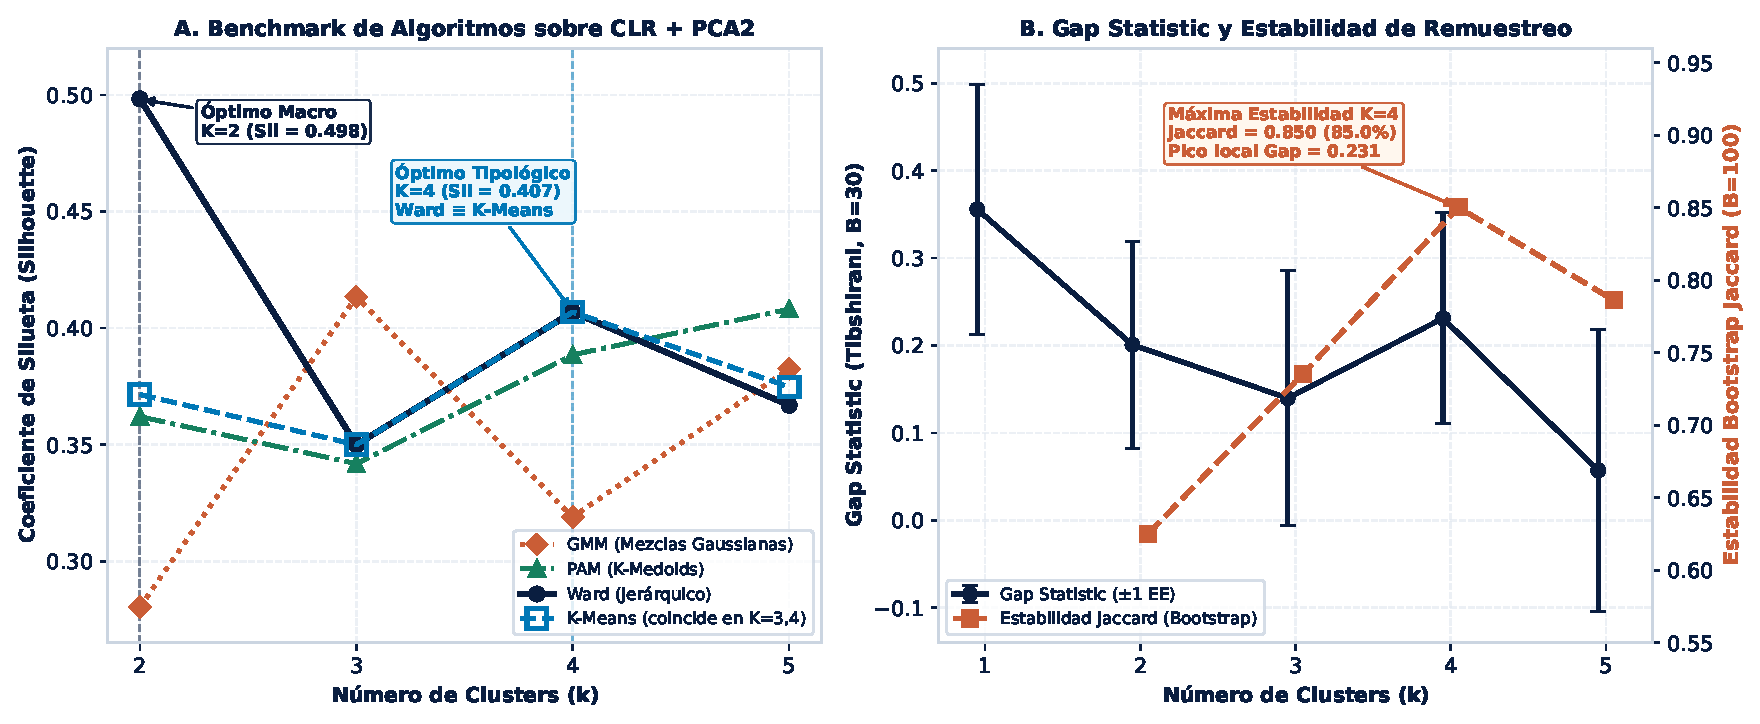
\includegraphics[width=0.88\textwidth,height=0.47\textheight,keepaspectratio]{figures/fig2_validacion_clustering.pdf}
\end{center}
\vspace{-0.24cm}
\begin{columns}[T,onlytextwidth]
\begin{column}{0.59\textwidth}
\begin{ccdebox}[left=2mm,right=2mm,top=0.8mm,bottom=0.8mm]
\scriptsize\RaggedRight
\textbf{Convergencia (48 modelos)}: En $K=4$ sobre CLR+PCA2, \textbf{Ward} y \textbf{K-Means} producen la misma partición ($\text{Silueta}=0.407$, $\text{CH}=22.24$), superando a PAM ($0.389$) y GMM ($0.319$).
\end{ccdebox}
\end{column}
\begin{column}{0.38\textwidth}
\begin{keybox}[left=2mm,right=2mm,top=0.8mm,bottom=0.8mm]
\scriptsize\RaggedRight \textbf{Doble Óptimo}: $K=2$ lidera en silueta ($0.498$) y $K=4$ maximiza estabilidad Jaccard ($85.0\%\text{--}87.7\%$).
\end{keybox}
\end{column}
\end{columns}
\source{Tibshirani et al.\ (2001) para Gap Statistic ($B=30$); Hennig (2007) para estabilidad Jaccard ($B=100$).}
\end{frame}

% ================================================================
\begin{frame}{Mapa Estructural: Cuatro Perfiles en CLR + PCA}
\vspace{-0.14cm}
\begin{columns}[c,onlytextwidth]
\begin{column}{0.65\textwidth}
\centering
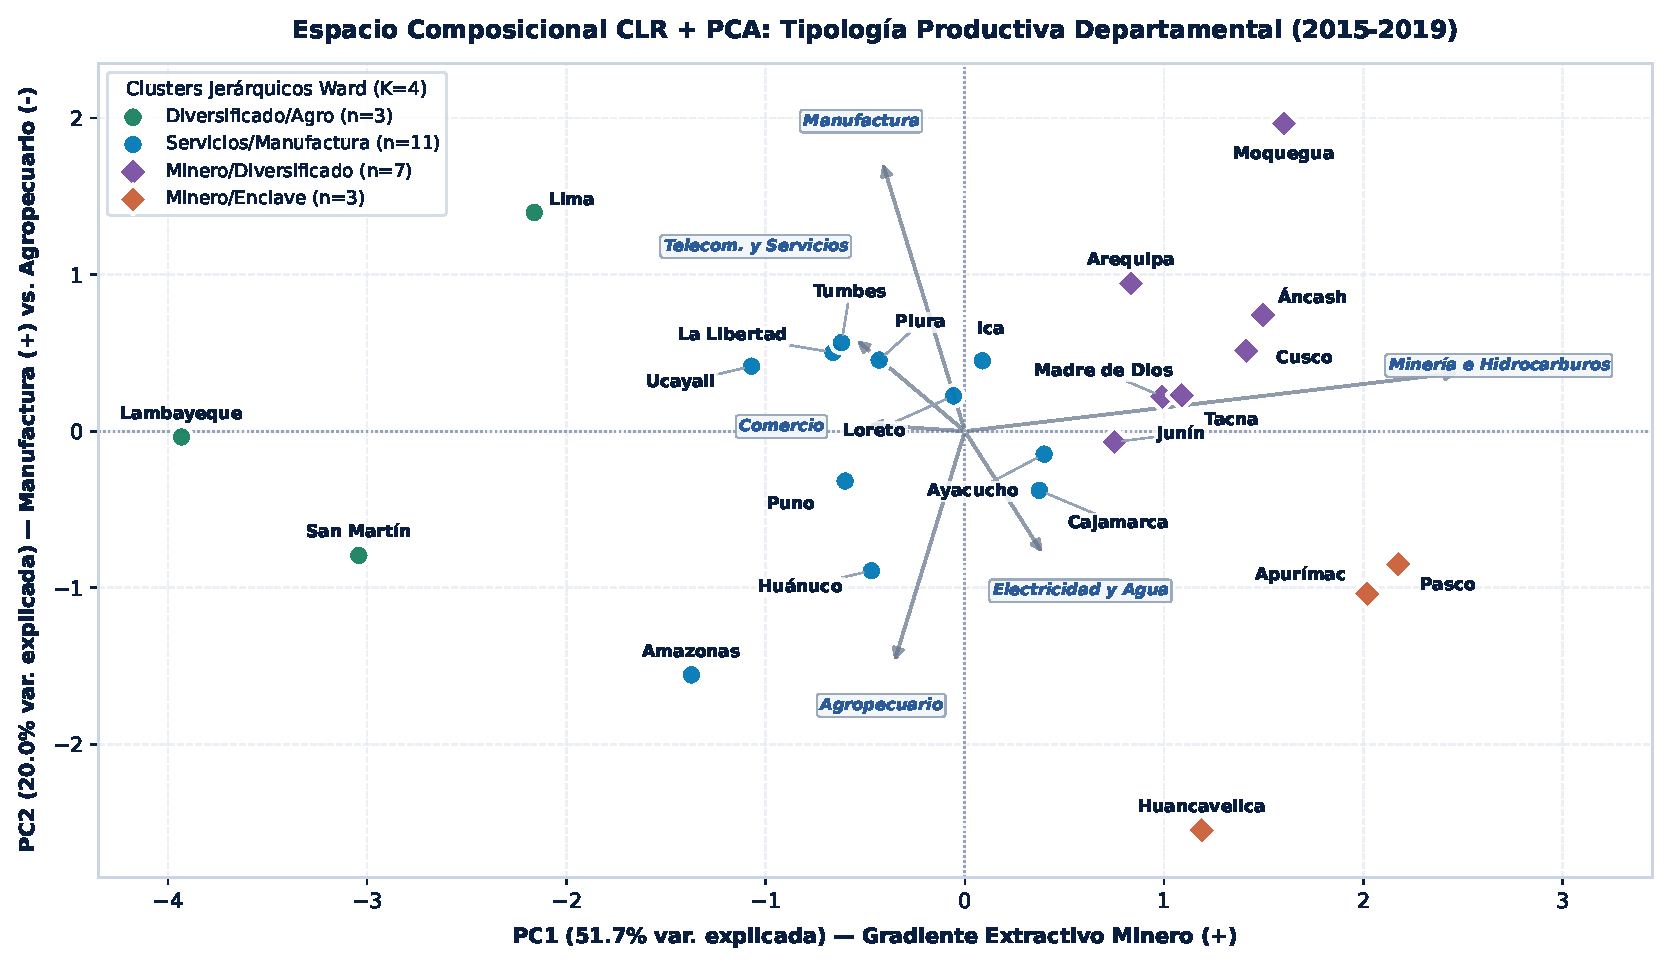
\includegraphics[width=\linewidth,height=0.66\textheight,keepaspectratio]{figures/fig1_pca_biplot_clusters.pdf}
\end{column}
\begin{column}{0.33\textwidth}
\begin{ccdebox}[left=2mm,right=2mm,top=1mm,bottom=1mm]
\scriptsize\RaggedRight
\textbf{\textcolor{ccdenavy}{Geometría de los 4 Clusters}}\\[0.05cm]
\textcolor{warn}{$\blacklozenge$ \textbf{Minero/Enclave ($n=3$):}}\\
Apurímac, Pasco y Huancavelica (alta extracción + energía).\\[0.05cm]
\textcolor{purplex}{$\blacklozenge$ \textbf{Minero/Diversificado ($n=7$):}}\\
Moquegua, Áncash, Cusco, Arequipa, Tacna, Madre de Dios y Junín.\\[0.05cm]
\textcolor{ccdeaccent}{$\bullet$ \textbf{Servicios/Manufactura ($n=11$):}}\\
Núcleo central (Ica, La Libertad, Piura, Cajamarca, Puno, etc.).\\[0.05cm]
\textcolor{okgreen}{$\bullet$ \textbf{Diversificado/Agro ($n=3$):}}\\
Lima, Lambayeque y San Martín en el extremo no minero ($PC1 < -2$).
\end{ccdebox}
\end{column}
\end{columns}
\source{Elaboración propia sobre el promedio composicional 2015--2019 (\texttt{modelo-clusters.ipynb}).}
\end{frame}

% ================================================================
\begin{frame}{Anatomía Jerárquica: $K=4$ Anidado dentro de $K=2$}
\vspace{-0.18cm}
\begin{center}
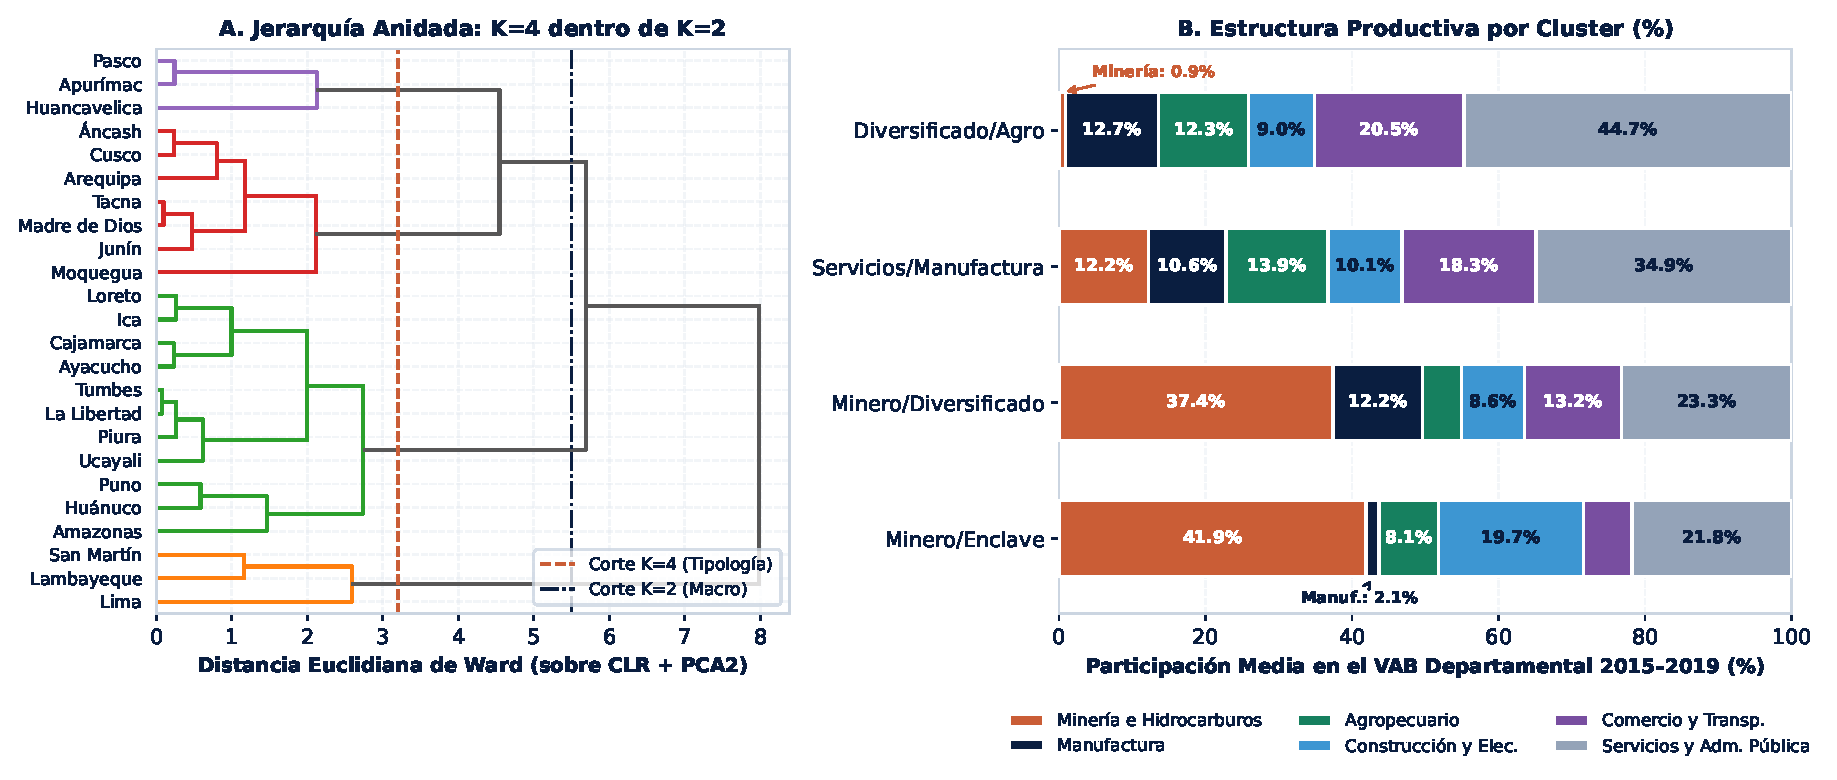
\includegraphics[width=0.90\textwidth,height=0.50\textheight,keepaspectratio]{figures/fig3_dendrograma_perfiles.pdf}
\end{center}
\vspace{-0.24cm}
\begin{keybox}[left=2mm,right=2mm,top=0.8mm,bottom=0.8mm]
\scriptsize\RaggedRight
\textbf{Anidamiento exacto de Ward}: Los 4 clusters se agrupan sin cruces en dos bloques macroeconómicos: \textbf{Bloque Minero} ($N=10$: \textit{Enclave} $41.9\%$ minería + \textit{Minero/Div.} $37.4\%$ minería) vs.\ \textbf{Bloque Diversificado} ($N=14$: \textit{Serv./Manuf.} $12.2\%$ + \textit{Div./Agro} $0.9\%$).
\end{keybox}
\source{Resultados en \texttt{clustering\_paso4\_perfil\_K4.xlsx} y \texttt{econ\_reagrupa.py}.}
\end{frame}
